\documentclass[a4paper,12pt]{article}
\usepackage{tikz}
\usetikzlibrary{automata}

\begin{document}
 \begin{center}
    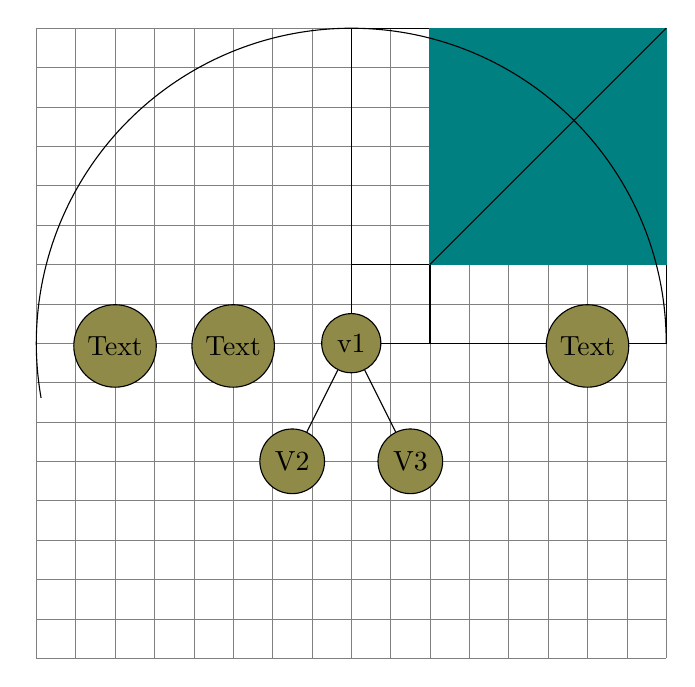
\begin{tikzpicture}[every node/.style={circle,draw=black,fill=yellow!50!black}]
        \draw[step=.5cm,gray,very thin] (-4,-4) grid (4,4);
        \draw (0,0) rectangle (4,4);
        \draw (1,1) rectangle (0,0);
        \filldraw[teal] (1,1) rectangle (4,4);
        \draw (4,0) arc [start angle=0,end angle=190,radius=4];
        \draw (1,1) -- (4,4);
        \foreach \x in {-1,-0.5,1}
        \draw[xshift=\x*3 cm] (0pt,-1pt) -- (0pt,1pt)
        (0pt,-1pt) node {Text}
        ;

        \node at(0,0){v1}
            child {node{V2}}
            child {node{V3}}
        ;
    \end{tikzpicture}  
   
 \end{center}
\end{document}
